

\begin{landscape}
 
 
 \begin{figure}[hp]
\centering
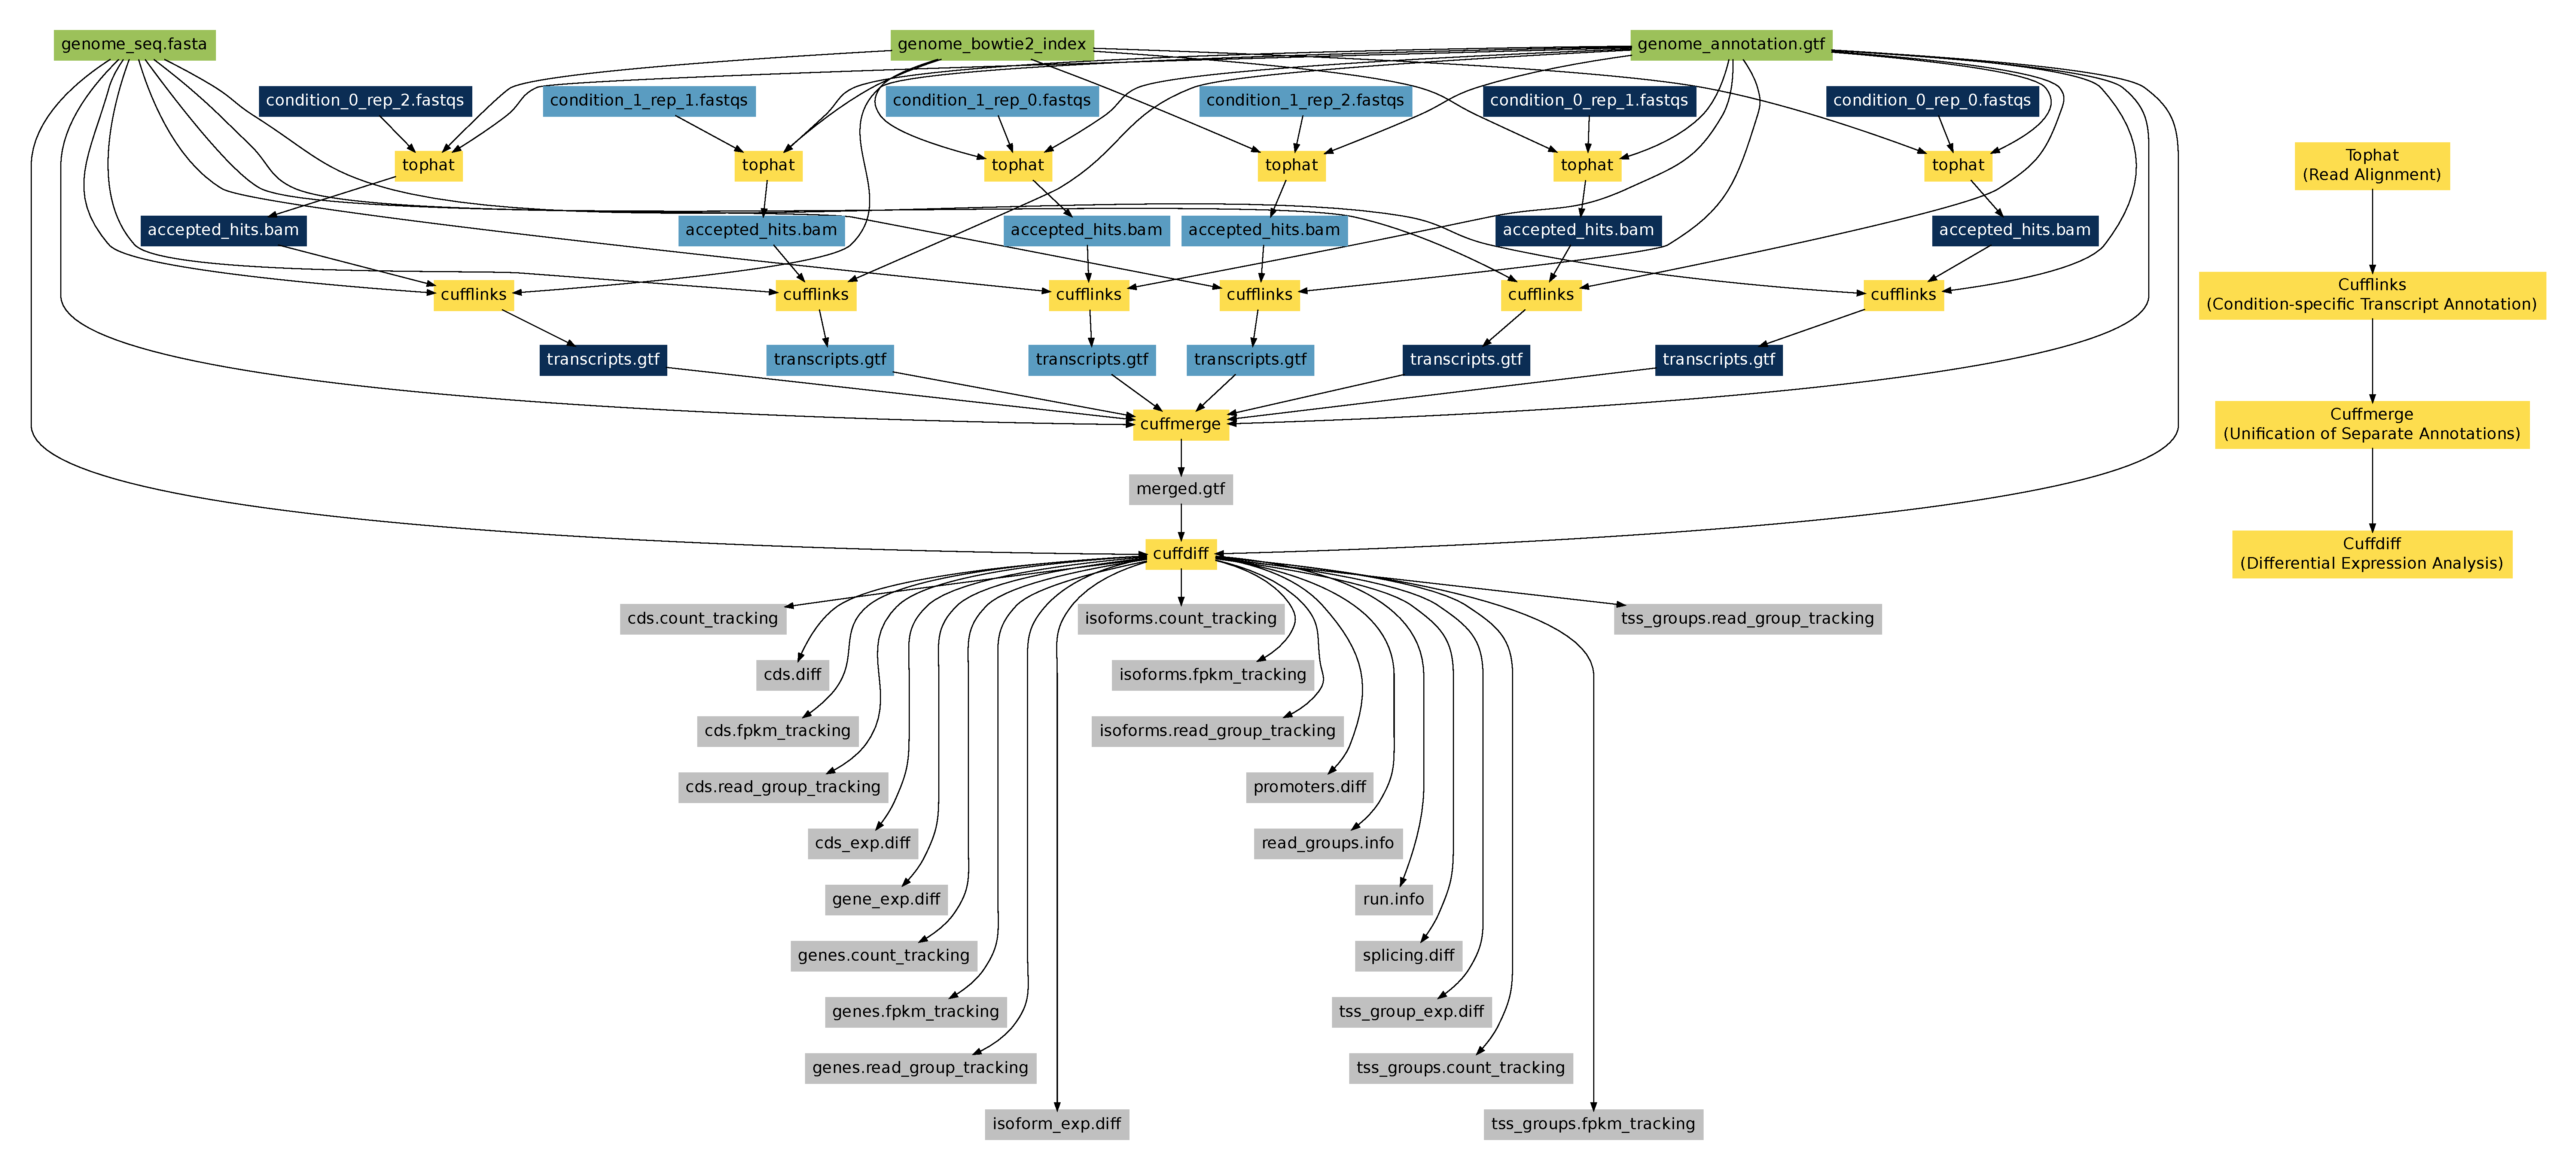
\includegraphics[width=\linewidth]{figures/figs/tuxedo_dot/707354_6/tophat_cufflinks_ins_outs.pdf}
\caption[Diagram of Abbreviated Tophat/Cufflinks Inputs and Outputs]{\textbf{Diagram of Abbreviated Tophat/Cufflinks Inputs and Outputs:}\\
	This figure demonstrates the complexities of a typical RNA-seq experiment as analyzed with the ``Tuxedo Protocol''. It models a fairly \textbf{simple} two condition experiment with each condition having three replications. It is ``abbreviated'' in that it only displays the output files that will be used in the next step for all steps except the \UseVerb{cuffdiff} step. The complete output of \UseVerb{cuffdiff} is included to demonstrate the final challenge of integrating the data which exists in multiple cross-referenced files.\\ 
	(\textsc{Dark Blue} - Inputs/Outputs associated with Condition Zero; 
	\textsc{Light Blue} - Inputs/Outputs associated with Condition One; 
	\textsc{Grey} - Inputs/Outputs associated with Condition Zero \textbf{AND} Condition One; 
	\textsc{Green} - Inputs Specific to the Reference Genome; 
	\textsc{Gold} - Program Calls)
}
	\label{fig:tuxedo}
\end{figure}
 
 
 
\end{landscape}

